\chapter{X-WikiRE}
\label{chpt:4}
\paragraph{}
Supervised training of deep neural networks often requires a large amount of high-quality training data which are difficult to obtain.  To fix this, ~\cite{hewlett2016wikireading} exploited Wikidata~\cite{vwikidata} and Wikipedia to create large amounts of distantly annotated data for various natural understanding tasks. \cite{levy2017zero} used WikiReading as a starting point for building a large scale reading-comprehension based dataset for relation extraction. We use these two works to build out multilingual reading-comprehension based dataset for relation extraction. X-WikiRE is available in the following languages: English, Spanish, Italian, German, and French.

In this chapter we will describe how we built X-WikiRE. First,  we will describe our datasources, Wikipedia and Wikidata. Next, we will describe the process we used to combine these resources to obtain annotated data for different languages. As final step, we will describe how to increase the number of examples by creating different templates. In the last section, we will show some descriptive statistics about X-WikiRE.


\section{Datasources}
\paragraph{}
Our datasources are Wikipedia, and Wikidata. Wikidata it's a free collaborative knowledge base that is available in more than 300 languages. It's value has long been obvious, with many efforts to use it. The Wikidata approach is to crowd source data acquisition, allowing a global community to edit it's content, making it a good quality resource.  Wikipedia is a online encyclopedia with articles available, as for Wikidata, in more than 300 languages..  %Wikidata provides dumps in different data formats, spanning from XML, Turtle, NTriples, and JSON. We choose the latter and describe below it's datamodel. Instead Wikipedia only provides XML dumps, which can be converted to JSON using existing tools\footnote{\url{https://www.mediawiki.org/wiki/Alternative_parsers}}, but we opted to scrape them since the output provided by these tools is sometimes too noisy or require some changes to allow the merge with Wikidata.

% The two used sources are are different in both size, and contained information. We can have a quick recap in Table~\ref{tab:datasets}. The next two sections will present a more in detail description of these resources.

% TODO ADD other languages stats.
% \begin{table}[h]
%     \centering
%     \begin{tabular}{l|l|l}
%          &  Wikidata & EN Wikipedia  \\ \hline
%     Documents  & 50M & 5.5M \\
%     Size & 730GB & 15GB \\
%     Information & Semi-structured & Unstructured \\
%     \end{tabular}
%     \caption{Dataset stats}
%     \label{tab:datasets}
% \end{table}

\paragraph{Wikidata}
We can see Wikidata as a collection of triples \texttt{(entity, property, value)}. Each entity is identified by a unique number, prefixed with the letter Q, known as a ``QID". Also properties, which define the relation between the entities, are identified by a prefix P and a number (e.g. ``\texttt{P35}" is the id for the property "\textit{head\_of\_state}"). The relations each entity holds with other entities are called \textit{statements}. Values could be either other entities, or numeric/textual values.  For example, given the entity \textit{Niels Bohr}, with id \texttt{Q7085}, the relation \textit{born\_in} (with id \texttt{P19}), and the entity \textit{Copenhagen}, id \texttt{Q1748}, we will have the triple \texttt{(Q7085, P19, Q1748)} stating that Niels Bohr was born in Copenhagen. Items may be linked to articles on Wikipedia.


% \paragraph{Wikipedia}
% Wikipedia is an online encyclopedia, it is structurated in articles, each one about a specific entity. 

\section{X-WikiRE}
X-WikiRE construction is based on WikiReading~\citep{hewlett2016wikireading} and~\citep{levy2017zero}. 




\subsection{Querification}


\begin{table}[h!]
\fontsize{10}{10}\selectfont
\centering

\begin{tabular}{p{0.75cm}p{4cm}p{10cm}}%{|p{1cm}|p{5cm}|p{9cm}|}
\toprule
Lang & Question                                                      & Context \& Answers                                                                                                                                                                                                                      \\ \midrule
DE       & In welchem land befindet man sich, wenn man \textbf{Amazonas} besucht? & Der Fluss Amazonas gab seinerseits dem Amazonasbecken sowie mehreren gleichnamigen Verwaltungseinheiten in \textbf{Brasilien}, \textbf{Venezuela}, \textbf{Kolumbien} \dots                                                                         \\ \midrule
EN       & What country is \textbf{Amazon} located in?                            & The Amazon proper runs mostly through \textbf{Brazil} and \textbf{Peru}, and is part of the border between \dots                                                                                                                             \\ \midrule
ES       & ¿En qué país se encuentra el \textbf{Amazonas}?                        & El río Amazonas es un río de América del Sur, que atraviesa \textbf{Perú}, \textbf{Colombia} y \textbf{Brasil}.                                                                                                                       \\ \midrule
FR       & Dans quel pays peux-tu trouver \textbf{Amazone}?                       & Le fleuve prend alors le nom d'Amazonas au \textbf{Pérou} et en \textbf{Colombie}, puis celui de rio Solimões en entrant au \textbf{Brésil} au \dots \\ \midrule
IT       & Di quale nazione fa parte il \textbf{Rio delle Amazzoni}?              & Il Rio delle Amazzoni è un fiume dell'America Meridionale che attraversa \textbf{Perù}, \textbf{Colombia} e \textbf{Brasile} \dots                                                                    \\ 
\bottomrule
\end{tabular}

\caption{Examples from our dataset of the same question-context pairs across all the languages with the correct answers highlighted in boldface.}
\label{table:qa_examples}
\end{table}

\section{Dataset Statistics}

\begin{table}[t!]
\fontsize{10}{10}\selectfont
\label{table:datasetstats}
\centering
\begin{tabular}{c | c c c c}
\toprule
Language & Pos  & Neg  & Pos*  & Neg* \\ \midrule
DE       & 2.5M & 545K & 11M  & 2.3M \\ %\hline
EN       & 5.1M & 1M   & 64M  & 12M  \\ %\hline
ES       & 1.2M & 211K & 5.5M & 1.1M \\ %\hline
FR       & 2.3M & 867K & 18M  & 6.8M \\ %\hline
IT       & 1.9M & 217K & 10M  & 1.2M \\ %\hline
\bottomrule

\end{tabular}
\caption{The number of positive and negative triples for each language with (*) and without templates.}
\label{data:stats}
\end{table}


\begin{figure}%[ht!]
\centering
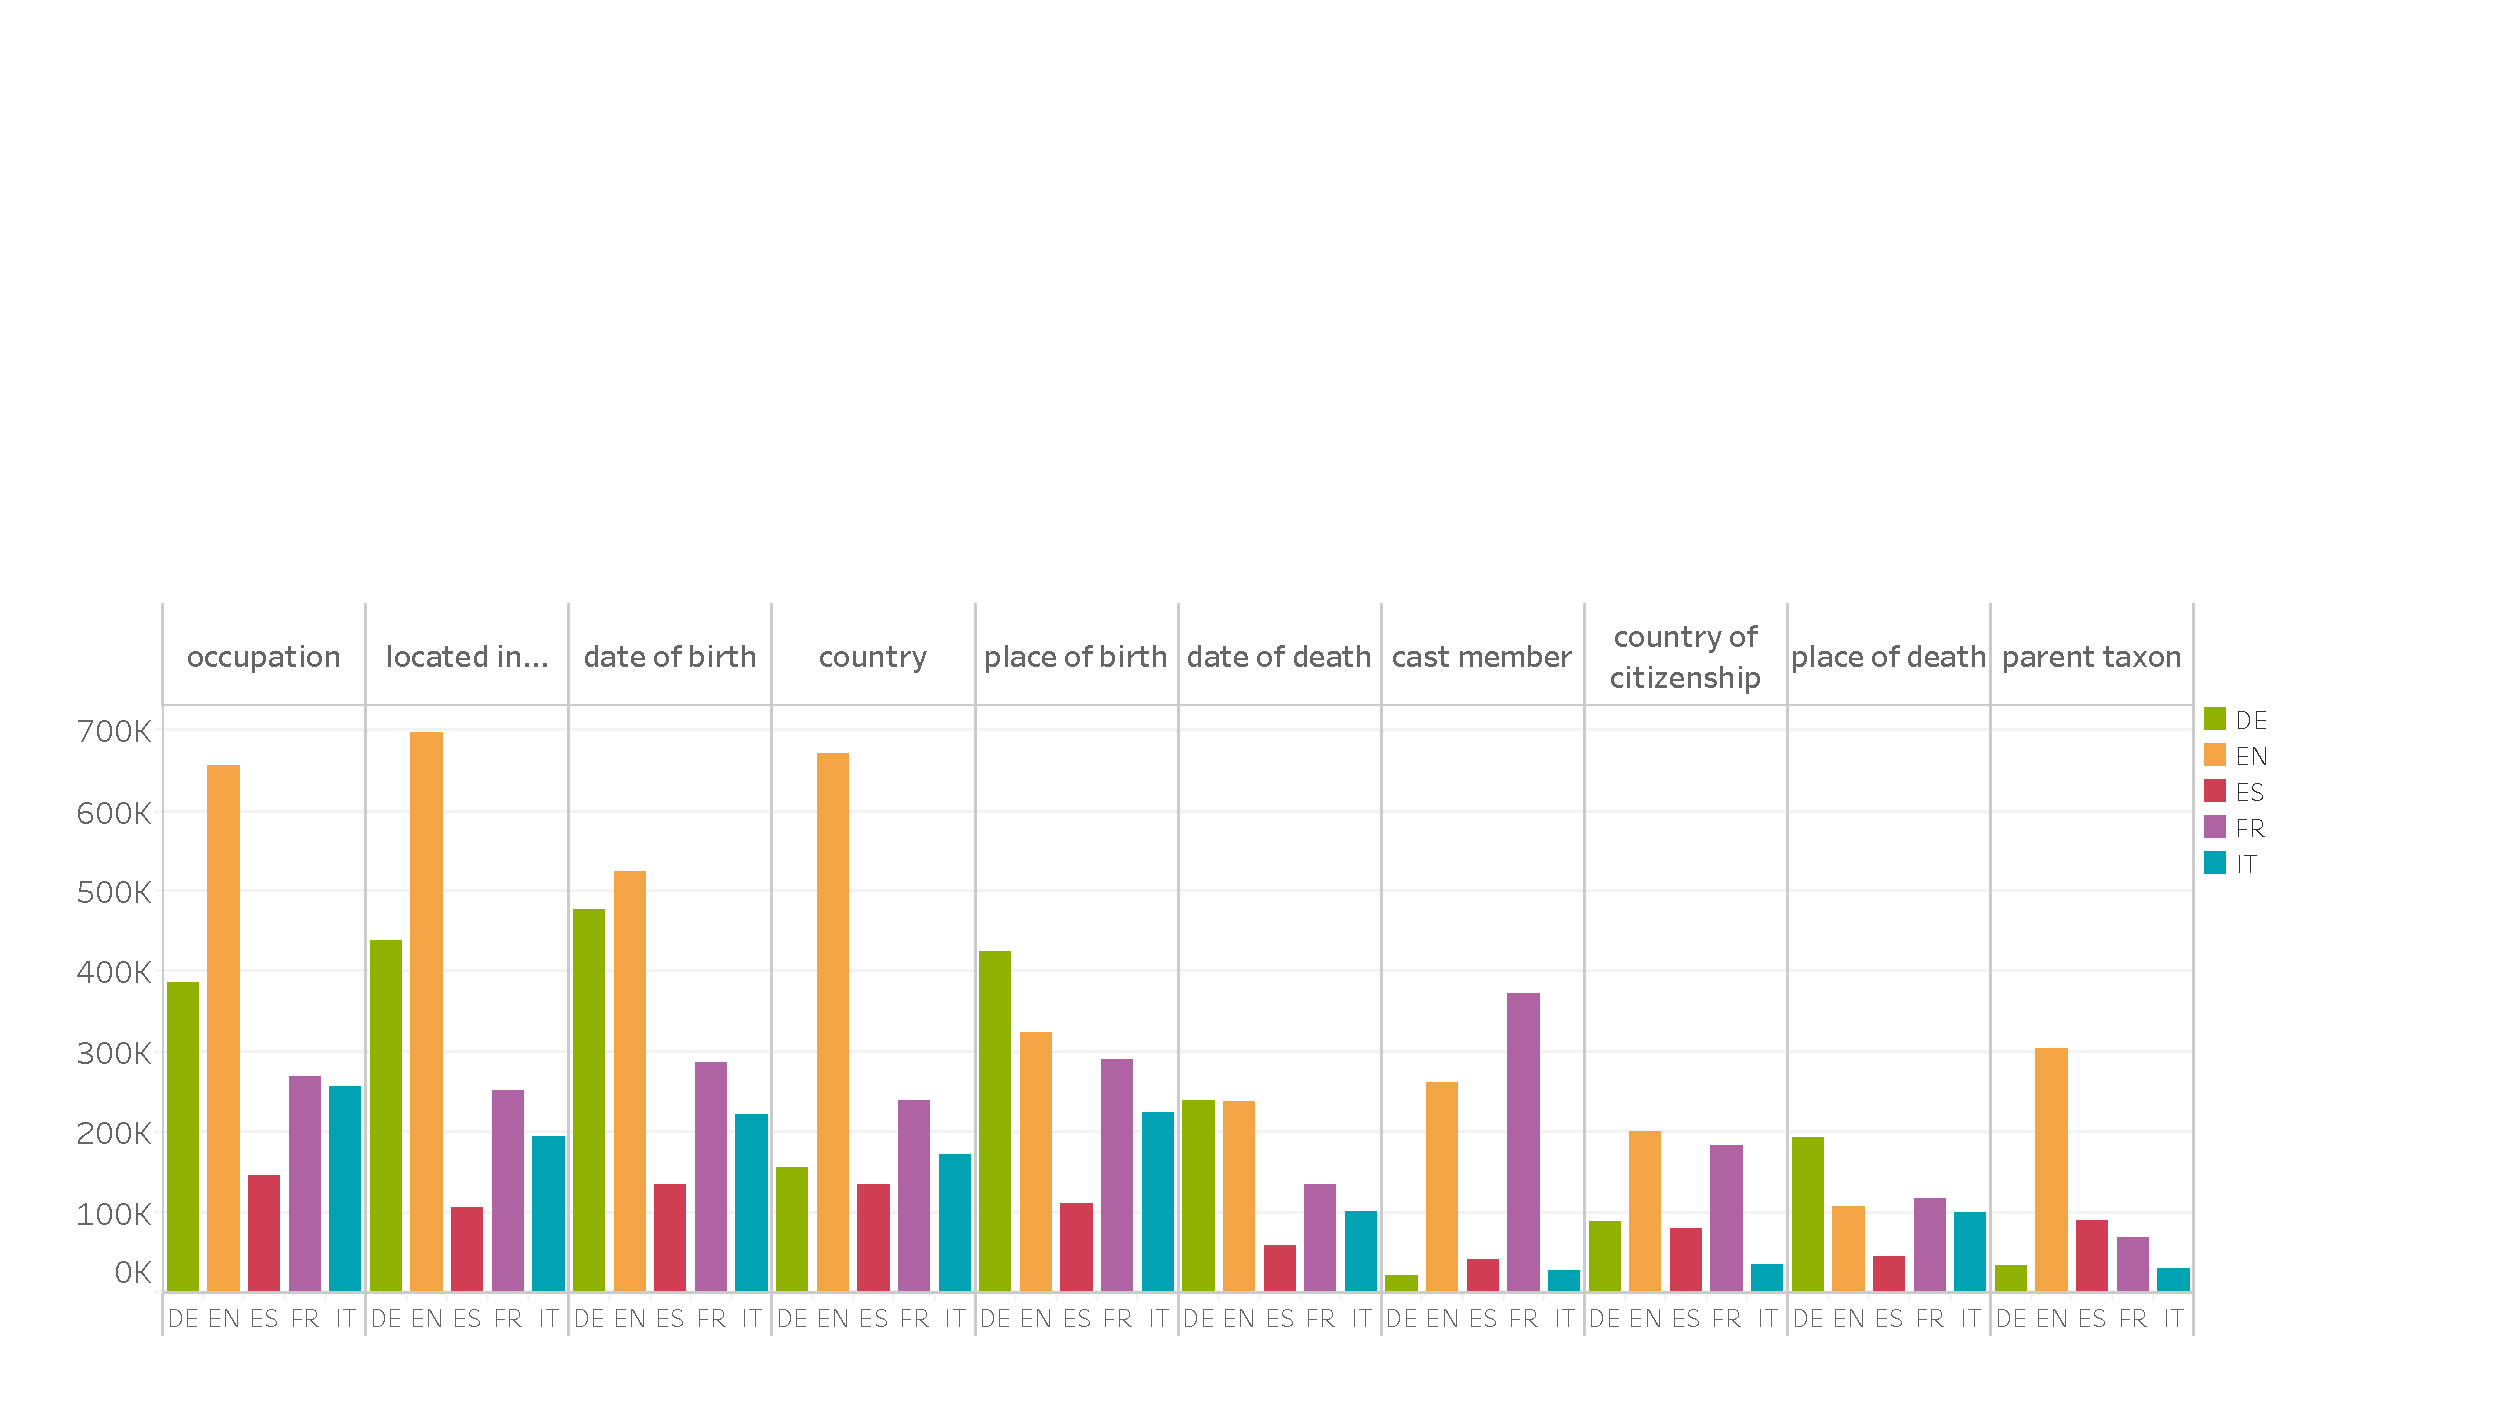
\includegraphics[width=\textwidth]{images/count_examples-property_per_language_wide.pdf}
\caption{The number of triples for the top 10 properties in each language.}
\label{fig:top_10}
\end{figure}